\section{Introduction}
\label{S:introduction}
We investigate the random vibrations of a nonlinear stochastically-forced system of the form
\begin{equation}
\begin{aligned} 
\ddot q_1(t) + \zeta_1 \dot q_1(t) + f_1(q_1(t),q_2(t)) &= \xi (t)\\
\ddot q_2(t) + \zeta_2 \dot q_2(t) + f_2(q_1(t),q_2(t)) &= 0
\end{aligned}
\qquad t \ge 0
\label{E:2dof}
\end{equation}
where for each time $t > 0$, $(q_1(t), q_2(t))$ represents the generalized coordinates of the system, the constants $\zeta_1$ and $\zeta_2$ are damping coefficients, and $\xi$ is a stationary random process. While only the first mode $q_1$ is forced, the nonlinear coupling can transfer energy to the second mode $q_2$. Often, systems such as~\eqref{E:2dof} are known as \emph{autoparametric systems} (one may think of $q_1$ as a parameter in the dynamics of $q_2$). Our focus here is when the dynamics of $q_1$ and $q_2$ are that of coupled and damped oscillators, and we are then interested in questions of \emph{stability} of the stochastic system~\eqref{E:2dof}, and in particular we are interested in the transfer of energy from the forced mode to the unforced mode.

% Describe general form of autoparametric systems

Periodically excited autoparametric systems have been studied extensively; see for example \citet{sethna65:_vibrat_of_dynam_system_with_qudrat_nonlin, haxton72:_autop_vibrat_absor, nayfeh79:_nonlin_oscil, hatwal83:_forced_nonlin_oscil_of_autop_1, bajaj96:_amplit_modul_dynam} and \citet{tien94:_nonlin_dynam_of_shall_arch}. The most interesting situations occur when the natural frequencies of the excited mode and the unexcited mode are in 2:1 resonance. If the excitation is periodic and the energy of the forced oscillator is increased, it reaches a certain value of amplitude at which saturation takes place for the oscillator and the energy is transferred to the unforced second mode. This may be undesirable, because disturbances affecting one mode may cause unwanted instability in another mode. Our effort (which is not considered by any of the above works) is to study energy transfer in the presence of noisy input.

A natural question is whether such saturation and transfer of energy take place in the presence of stationary random excitations (as opposed to deterministic periodic excitations). Although various papers have dealt with some aspects of this question, non have given completely satisfactory answers. This is primarily due to the complex interactions between, noise, nonlinearities and resonances. Our approach is to study these interactions via a \emph{novel dimensional-reduction} approach. The analysis hinges upon some recent abstract theories of stochastic dimensional reduction. We then use this reduced model to calculate some essential design-related statistical measures of response and stability (e.g., mean exit times and stationary measures).

The important assumption in our analysis is that the dissipation and random perturbations are small. Of course this means that their effect will be visible only over a long time horizon. However, since the noise is small, the dynamics of the unperturbed system gives some structure to our analysis and organizing the effects of the random perturbation. In particular, the dynamics of the unperturbed system identify a reduced phase space (the orbit space) on which to carry out stochastic averaging. While the classical theory of stochastic averaging is a natural framework for such a program, the equations of interest contain resonances and bifurcations, which precludes a simple application of classical techniques. In particular, the resonance gives rise to an intermediate scale, and the bifurcations give rise to some non-standard singularities in the orbit space. See \citet{freidlin94:_random_pertur_of_hamil_system,freidlin98:_random_pertur_nonlin_oscil,namachchivaya01:_non_duffin_pol} and \citet{sowers02:_stoch_averag_with_flatt_hamil} for some related investigations.

\section{Physical Model}
\label{S:model}

The equations of motion~\eqref{E:2dof} considered can model the dynamics of a number of structural and mechanical systems, namely a randomly excited and initially deformed shallow arch, a suspended elastic cable driven by planar excitation, or a water vessel subject to longitudinal wave action. To keep things as simple as possible, we shall consider a very simple system, namely a type of \emph{autoparametric vibration absorber with randomly excited base} (see \citep{hatwal83:_forced_nonlin_oscil_of_autop_1}). Namely, we shall consider a mass attached by a spring to a pendulum, as illustrated in Figure~\ref{F:ap schematic}. For clarity, we use \emph{mass} to refer to the object at the free end of the spring, while the object at the end of the pendulum is referred to as the \emph{bob}. The quantity $\varphi$ is the angle of the pendulum (with respect to the vertical axis) and the quantity $y$ represents the height of the mass (relative to a rest position defined by the position of the pendulum). The mass is forced according to a stochastic signal $\Xi(t)$. The subscripts here refer to the fact that this is our original physical model. The equations for such a system can be written as
\begin{equation}
\label{e:absorber}
\begin{gathered}
(m_o + m_p) \ddot y + d_o \dot y + k y + m_p l (\ddot \varphi \sin \varphi + {\dot \varphi}^2 \cos \varphi) = \Xi\\
m_p l^2 \ddot \varphi + d_p \dot\varphi + m_p l (g + \ddot y) \sin \varphi = 0
\end{gathered}
\end{equation}
where $m_o$, $d_o$ and $k$ are the mass, damping and the spring constant of the spring-mass system and $m_p \,$, $d_p$ and $l$ are the mass, damping and the length of the pendulum.
\begin{figure}
\begin{center}
\psfrag{k}{$k$}
\psfrag{d}{$d$}
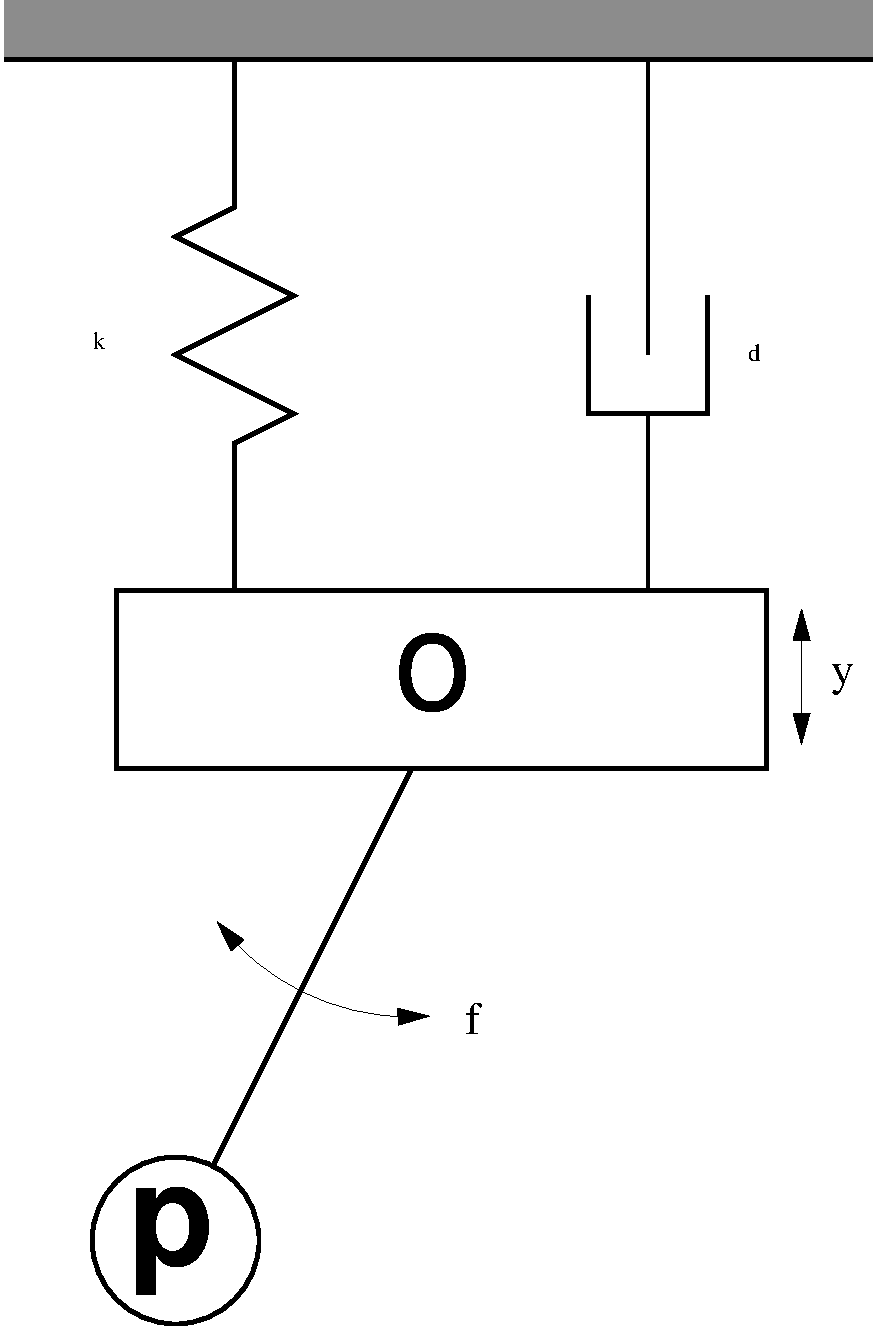
\includegraphics[width=\textwidth*7/8]{figures/autoparam_schematic}
\caption{Schematic of the autoparametric system governed by equations~\eqref{e:absorber}. The letter ``o'' denotes the mass and ``p'' denotes the pendulum.}
\label{F:ap schematic}
\end{center}
\end{figure}
The kinetic and the potential energies of the conserved system are given by
\begin{gather*}
T \equiv \frac12 (m_o + m_p){\dot y}^2 + \frac12 m_p \, l^2 {\dot \varphi}^2 + m_p \, l \dot y \, \dot \varphi \sin \varphi\\
U \equiv m_p \, g l ( 1 -\cos \varphi) + \frac12 k y^2
\end{gather*}
It is clear that the nonlinearities in the equations of motion arise due to the gravitational restoring force and due to the dependence of kinetic energy on the angle $\varphi$ which leads to inertial coupling between the the two coordinates. It also turns out (we shall use this later) that in the absence of noise and damping, this system is Hamiltonian, so the dynamics of $y$ and $\varphi$ are governed by the geometry of this Hamiltonian.

In order to non dimensionalize the equations in system \eqref{e:absorber}, a change of variables is introduced:
\begin{align*}
t &= \tau/\omega_0, & y(t) &= l \hat \eta(\tau), & \varphi(t) &= \hat \theta(\tau), & \Xi(t) &= k l \hat \xi(\tau).
\end{align*}
$\omega_o$ is defined by
\[
\omega_o^2 = \frac{k}{m_o + m_p}
\]
Then
\begin{align*}
\frac{dy(t)}{dt} &= l \frac{d \hat \eta(\tau)}{d \tau} \frac{d \tau}{d t}\\
&= l \omega_o \frac{d \hat \eta(\tau)}{d \tau}
\end{align*}
\[
\frac{d^2y(t)}{dt^2} = l \omega_o^2 \frac{d^2 \hat \eta(\tau)}{d \tau^2}
\]
\[
\frac{d \varphi(t)}{dt} = \omega_o \frac{d \hat \theta(\tau)}{d \tau}
\]
\[
\frac{d^2 \varphi(t)}{dt^2} = \omega_o^2 \frac{d^2 \hat \theta(\tau)}{d \tau^2}
\]
Substituting into the equation for $y$ in \eqref{e:absorber} gives
\[
\ddot{\hat \eta} + \frac{d_o}{\sqrt{k}\sqrt{m_o + m_p}} \dot{\hat \eta} + \hat \eta + \frac{m_p}{m_o + m_p} (\ddot{\hat \theta} \sin \hat \theta + {\dot{\hat \theta}}^2 \cos \hat \theta) = \hat \xi
\]
Two dimensionless quantities follow naturally:
\begin{align*}
\hat \zeta_o &= \frac{d_o}{2 \sqrt{k} \sqrt{m_o + m_p}} & R &= \frac{m_p}{m_o + m_p}
\end{align*}
The equation for $\ddot{\hat \eta}$ becomes
\[
\ddot{\hat \eta} + 2 \hat \zeta_o \dot{\hat \eta} + \hat \eta + R(\ddot{\hat \theta} \sin \hat \theta + {\dot{\hat \theta}}^2 \cos \hat \theta) = \hat \xi
\]
The equation for $\varphi$ when non dimensionalized becomes
\[
m_p l^2 \omega_o^2 \ddot{\hat \theta} + d_p \omega_o \dot{\hat \theta} + m_p l^2 \omega_0^2 (\frac{g}{l \omega_o^2} + \ddot{\hat \eta}) \sin \hat \theta = 0.
\]
Substituting for $\omega_o$, $\omega^2 = g/l$ and $q = \omega/\omega_o$ gives
\[
R \ddot{\hat \theta} + \frac{d_p}{l^2 \sqrt{k} \sqrt{m_o + m_p}} \dot{\hat \theta} + R (q^2 + \ddot{\hat \eta}) \sin \hat \theta = 0
\]
Introducing a third nondimensional quantity:
\[
\hat \zeta_p = \frac{d_p \sqrt{m_o + m_p}}{2 l^2 m_p \sqrt{k}} = \frac{d_p}{2 l^2 m_p \omega_o},
\]
the equation for $\hat \theta$ becomes
\[
R \ddot{\hat \theta} + 2 R \hat \zeta_p \dot{\hat \theta} + R (q^2 + \ddot{\hat \eta}) \sin \hat \theta = 0
\]
The corresponding Lagrangian for the autonomous and non-dissipative system is
\begin{equation}
\label{E:lagrangian}
L = \frac12 {\dot{\hat\eta}}^2 + \frac12 R {\dot{\hat\theta}}^2 + R {\dot{\hat\eta}}\,{\dot{\hat\theta}}\,\sin \hat{\theta} - \frac12 {\hat \eta}^2 - R q^2 \left(1 - \cos \hat{\theta} \right)
\end{equation}
Making use of the velocities in terms of the generalized momentum, we
have
\begin{equation}
\label{E:velocity}
\dot {\hat \eta} = \frac {p_1 - p_2\,\sin \hat{\theta} }{1-R \sin^2 \hat{\theta} },\quad \dot {\hat \theta} = \frac {p_2- R \, p_1\,\sin \hat{\theta} }{R\left(1- R \sin^2 \hat{\theta} \right)}
\end{equation}
and from Legendre transformation we obtain the Hamiltonian as
\[
H = \frac12 \frac{{p_1}^2}{1 - R \sin^2 \hat{\theta}} - \frac{p_1 p_2 \sin \hat{\theta}}{1- R \sin^2\hat{\theta}} + \frac12 \frac{{p_2}^2}{R (1 - R \sin^2\hat{\theta})} + \frac12 \hat{\eta}^2 + R q^2 (1 - \cos\hat{\theta}).
\]
When $\hat\xi$ is periodic, the motion of the mass causes variations in the absorber spring stiffness, and in turn, the absorber acts (in a nonlinear fashion) back on the main mass. With appropriate choice of tuning parameters, the effect of the mass can be completely absorbed. For periodically excited autoparametric systems, the most interesting situations occurs when the natural frequencies of the mass and the pendulum are in $2:1$ internal resonance; i.e., when $q = 1/2$. In resonance, the pendulum is primarily excited by energy coming from the mass. When the external energy put into the mass is small enough, its effect on the pendulum is small compared to the stability of the hanging pendulum. As the external energy increases, a saturation takes place at a certain threshold, above which the pendulum noticeably moves; see \citep{nayfeh79:_nonlin_oscil}. In some mechanical absorbers, this transfer of energy is useful. In other systems, it may not, since a disturbance affecting one mode may cause unwanted dynamics in other modes (for example, longitudinal wave action could lead to capsizing of a ship). Since such disturbances often contain an essential \emph{random} component (think of water waves in the ocean), it is essential to complement the above investigations of the effect of periodic excitations by corresponding investigations of the effect of random excitations.

Our interest here is a refined stability analysis near the fixed point $(\hat\eta,\hat\theta)\equiv 0$ of the unperturbed system. In particular, we are interested in the effect of small random perturbations, so we will let $\hat\xi$ be of the form $\hat\xi = \epsilon^2 \nu \xi$, where $\xi$ is a noise process of ``unit'' variance and $\nu$ is some empirical parameter. Our dynamics are most interesting when they are not overdamped, so let $\hat\zeta_o$ and $\hat\zeta_p$ be of the form $\hat\zeta_o = \epsilon^2 \zeta_o$ and $\zeta_p = \epsilon^2 \zeta_p$, where $\zeta_o$ and $\zeta_p$ are some positive constants (this corresponds to letting $d_o$ and $d_p$ be of size $\epsilon$). Guided by the corresponding analysis for periodic forcing, we are interested in the behavior when $q^2$ is very close to $q^2_o\equiv 1/4$. Let's replace $q$ by $q_o + \epsilon^2 \mu$, where $\mu$ is an unfolding parameter. Since we are interested in $\hat\eta$ and $\hat\theta$ near the fixed point $0$, we should look at these quantities on a finer resolution. Namely, let $\eta$ and $\theta$ be defined by
\[
\hat\eta(t) = \epsilon \eta(t) \qquad \hat\theta(t) = \epsilon \theta(t)
\]
Then the dynamics of our system are
\begin{equation}
\begin{aligned} 
\ddot \eta + 2 \epsilon^2 \zeta_o \dot \eta + \eta + R (\ddot\theta \sin(\epsilon\theta) + \epsilon \dot\theta^2 \cos (\epsilon\theta) ) &= \epsilon\nu\xi\\
\ddot \theta + 2 \epsilon^2 \zeta_p \dot \theta + \left( \left(q_o + \epsilon^2 \mu\right)^2 \frac{\sin (\epsilon \theta)}{\epsilon} + \ddot \eta \sin (\epsilon\theta) \right) &= 0.
\end{aligned}
\label{E:dynamics}
\end{equation}

The salient feature of this system is that the dominant deterministic component of the dynamics gives us a place to start to search for structure in the light of randomness. Once we understand this structure, we can then investigate how various system parameters (i.e., the damping coefficients, $R$, $\nu$ and $\mu$) affect various important engineering quantities -- exit times from stable regions, invariant measures, etc.

\section{Single Mode Solutions}
\label{S:single}

To clarify some general qualitative effects of noise, let's consider a simple stability analysis using some spectral methods and the first-order linearization. Assume that initially the pendulum hangs vertically, at rest. Then $\theta$ will be identically zero -- ``locked-mass'' dynamics. The mass on the spring can move only in the vertical direction and is excited by $\nu \xi$. We get the equation
\[
\ddot \eta + 2 \epsilon^2 \zeta_o \dot \eta + \eta = \epsilon \nu \xi.
\]
If $\xi$ is white noise we can solve for $\eta$ explicitly. Its power spectral density is
\[
S_\eta(\omega)=\frac{\epsilon^2\nu^2 S_0}{(1-\omega^2)^2+4\epsilon^4\zeta_o^2 \omega^2}
\]
where $S_0$ is the power spectral density of $\xi$. The peak intensity and the carrying frequency of $\eta$ are determined by the filter parameter $\zeta_o$.

The stability of the locked mass steady-state oscillation is now obtained by using the first-order approximation of sine and cosine in the dynamics for $\theta$. We get
\[
\ddot \theta + 2 \epsilon^2 \zeta_p \dot \theta + ( (q_0+\epsilon^2\mu)^2 + \epsilon \ddot \eta ) \theta =0
\]
and the power spectral density of $\ddot\eta$ is given by
\[
S_{\ddot \eta} (\omega) = \frac {\omega^4 \epsilon^2 \nu^2 S_0}{(1 - \omega^2)^2 + 4 \epsilon^4 \zeta_o^2 \omega^2}
\]
The maximal Lyapunov exponent can now be easily calculated and the stability boundary can be obtained in terms of excitation intensity $\nu$ and the dissipation coefficients $\zeta_p$. An explicit expression for the maximal Lyapunov exponents of the single mode solution is given
in \citet{arnold86:_asymp_analy_lyapun_expon} and \citet{namachchivaya87:_stoch_pertur_hopf_bifur}; expanding it in $\epsilon$, we have
\[
\lambda_1 \approx \epsilon^2 \left( - \zeta_p + \frac{1}{8 \, q_o^2} S_{\ddot \eta}(2 \,(q_o+\epsilon^2\mu))\right)
\]
Using the trace formula, the second Lyapunov exponent can be obtained as
\[
\lambda_2 = \epsilon^2 \left( - \zeta_p - \frac{1}{8 \, q_o^2} S_{\ddot \eta}(2 \,(q_o+\epsilon^2\mu)) \right).
\]
The noise has no effect on the other two exponents; i.e., $\lambda_3=\lambda_{4}= - \zeta_o$.

At exact one-to-two resonance, i.e., $\mu=0$, the maximal Lyapunov exponent reduces to
\begin{equation}
\lambda_1 = \epsilon^2 \left( - \zeta_p + \frac{{\nu}^2 \, S_0}{8 \, \zeta_o^2} \right)
\end{equation}
It is clear, that when the noise intensity $\nu^2$ is small (remember that we have normalized so that $\xi$ has unit intensity), the size of the oscillations of $\eta$ is similarly small. Since the point $\theta\equiv 0$ is a stable point for the hanging pendulum, the pendulum undergoes small random motion near $\theta\equiv 0$, and all four Lyapunov exponents are negative. However, as we further increase the noise intensity, the top exponent becomes positive when $\nu^2 S_0 = 8 \zeta_o^2 \zeta_p$. The system then becomes unstable, and a host of questions arise.
\begin{itemize}
\item Do both the mass spring oscillator and the pendulum undergo random vibrations when the top exponent becomes positive~(i.e., ${\nu}^2 \, S_{0} > 8\,\zeta_o^2\,\zeta_p$), i.e., does a new coupled-mode ``stationary solution'' or ``stationary density function'' appear?
\item Does the positive exponent lead to a transfer of energy from the mass to the vertically hanging pendulum, i.e., is the energy transferred only after the mean square amplitude of the motion of the mass reaches a certain critical size?
\end{itemize}

\section{Coupled Mode Problem}
\label{S:statement}

The deficit of the above analysis is that it relied upon simplifying linearizations. The true dynamics of $y$ and $\theta$ are of course globally governed by nonlinear effects. It is to an analysis of these nonlinear effects that we commend ourselves in this paper. Namely, in order to maintain the nonlinear nature of the dynamics of $y$ and $\theta$, we will keep all terms which are of order $\epsilon^2$ and larger.

Before writing out the exact equations, let's invoke some of the formalism of mechanics. We can rewrite~\eqref{E:dynamics} in terms of the generalized coordinates ($\eta, \theta$) and conjugate momenta ($p_1, p_2$) are expressed as
\[
\begin{aligned}
\dot \eta &= \frac{p_1 - p_2\sin (\epsilon \theta)}{1-R\sin^2(\epsilon \theta)}\\
\dot \theta &= \frac{p_2 - Rp_1\sin (\epsilon \theta)}{R(1-R\sin^2(\epsilon \theta))} \\
\dot p_1 &= -\eta - 2 \epsilon^2 \zeta_o\left(\frac{p_1 - p_2\sin (\epsilon \theta)}{1-R\sin^2(\epsilon \theta)}\right) + \epsilon \nu \xi\\
\dot p_2 &= R\epsilon \left(\frac{p_1 - p_2\sin (\epsilon \theta)}{1-R\sin^2(\epsilon \theta)}\right)\left(\frac{p_2 - Rp_1\sin (\epsilon \theta)}{R(1-R\sin^2(\epsilon \theta))}\right)\cos(\epsilon \theta) \\
&\qquad - R (q_0 + \epsilon^2 \mu)^2\frac{\sin (\epsilon \theta)}{\epsilon} - 2 \epsilon^2 R \zeta_p \left(\frac{p_2 - Rp_1\sin (\epsilon \theta)}{R(1-R\sin^2(\epsilon \theta))}\right)
\end{aligned}
\]
Expanding the sines and cosines and keeping terms up to order $\epsilon^2$, we get the system
\begin{gather*}
\dot \eta = p_1 - \epsilon p_2 \theta + \epsilon^2 R p_1 \theta^2\\
\dot \theta = \frac{p_2}{R} - \epsilon p_1 \theta + \epsilon^2 p_2 \theta^2\\
\dot p_1 = -\eta - 2 \epsilon^2 \zeta_o p_1 + \epsilon \nu \xi\\
\dot p_2 = -R q_0^2 \theta + \epsilon p_1 p_2 + \epsilon^2 \left\{\frac{1}{6} R q_0^2 \theta^3 - 2 R q_0 \mu \theta - R p_1^2 \theta - p_2^2 \theta - 2 \zeta_p p_2\right\}
\end{gather*}
and the Hamiltonian is
\begin{multline*}
\label{e:hamiltonian}
H = \frac{p_1^2}{2} + \frac{p_2^2}{2R^2} + \frac{\eta^2}{2} + \frac{Rq_0^2\theta^2}{2} - \epsilon p_1 p_2 \theta\\ + \epsilon^2\left\{\frac{p_2^2 \theta^2}{2} + \frac{R p_1^2\theta^2}{2} - \frac{R q_0^2 \theta^4}{24} + R q_0 \mu \theta^2 \right\}
\end{multline*}
The dominant dynamics of $\eta$ and $\theta$ are
\[
\ddot \eta + \eta = 0 \qquad \text{and}\qquad \ddot \theta + q_0^2 \theta = 0
\]
We apply the following time dependent symplectic transformation:
\begin{gather*}
\eta = x_1 \cos t + x_3 \sin t\\
p_1 = -x_1 \sin t + x_3 \cos t \\
\theta = [x_2 \cos (q t) + x_4 \sin (q t)]/\sqrt{R q}\\
p_2 = \sqrt{R q}\, [-x_2 \sin (q t) + x_4 \cos (q t)]
\end{gather*}
The conjugate pairs are $(x_1,x_3)$ and $(x_2,x_4)$. Then $\boldsymbol x = (x_1,x_2,x_3,x_4)$ satisfies the random evolution equation
\begin{equation}
\dot{\bm x}^\epsilon_t = \epsilon \bm b^1(\bm x^\epsilon_t,t) + \epsilon^2 \bm b^2(\bm x^\epsilon_t,t:\zeta,\mu) + \epsilon \bm \sigma(\bm x^\epsilon_t, t: \nu) \xi(t)
\label{E:standard1}
\end{equation}
where $b^1$ contains spatially quadratic nonlinearities (which come from a cubic Hamiltonian) and $b^2$ contains spatially cubic nonlinearities (arising from a quartic Hamiltonian), and terms arising from dissipation and detuning. The explicit form of the quadratic and cubic nonlinear terms are given in Appendix~\ref{A:autoparam nonlin vec fields}. The stochastic forcing terms are defined by
\[
\bm \sigma(x,t:\nu) = \{-\nu \sin t, 0, \nu \cos t, 0\}
\]

It is important to realize that there are three scales in~\eqref{E:standard1}. The periodicity of the coefficients appears on time intervals of order $1/\epsilon$. The terms containing $b^2$ and $\sigma$ cause fluctuations of order $\epsilon$ and $\sqrt{\epsilon}$. The effect of the $b^1$ term is to cause fluctuations of order 1. Our interest here is when the periodic fluctuations of the coefficients in a sense cancel out the fluctuations due to $b^1$, leaving us with fluctuations of order $\epsilon$.

\subsection{Conserved Quantities}
\label{S:averagedequations}

From the explicit formulas for $b^1$ in Appendix~\ref{A:autoparam nonlin vec fields} (where $q=1/2$), we see that for $x = (x_1,x_2,x_3,x_4) \in \reals^4$,
\[
(\Tave b^1)(x) =
\begin{pmatrix}
-\frac12 x_2x_4 \\
\frac12 (x_1 x_4 - x_2 x_3)\\
\frac14 (x_2^2-x_4^2)\\
\frac12 (x_1 x_2 + x_3 x_4)
\end{pmatrix}
\]
The Hamiltonian associated with these dynamics is
\begin{equation}
\label{E:Hamiltonian}
K(\boldsymbol x) = \frac14 x_1(x_4^2 - x_2^2) - \frac12 x_2 x_3 x_4
\end{equation}
The Hamiltonian system
\begin{equation}
\label{E:flow}
\dot{z} = \bar{\nabla} K(z)
\end{equation}
has a second integral which is in involution with the Hamiltonian \eqref{E:Hamiltonian} (two integrals of motion are in involution if their Poisson bracket vanishes identically). Thus, the unperturbed four-dimensional Hamiltonian has \emph{two first integrals in involution}, namely, the Hamiltonian itself \eqref{E:Hamiltonian} and a second invariant or constant of motion (momentum variable)
\begin{equation}
\label{E:momentum}
I(x) = (x_1^2+x_3^2)+\frac12\,(x_2^2+x_4^2).
\end{equation}
The invariant $I$ is functionally independent of $K$, exists globally and is single valued. 

\subsection{Structure of the Unperturbed Systems}
\label{S:Unperturbed}

Our main analytical tool is a certain method of \emph{dimensional reduction} of nonlinear systems with symmetries and small noise. As the noise becomes asymptotically small, one can exploit symmetries and a separation of scales to use well-known methods (viz. stochastic averaging) to find an appropriate lower-dimensional description of the system.

Consider the following symplectic transformation
\begin{align*}
x_1 &= \sqrt{2 J}\sin(\phi + 2 \psi) & x_3 &= \sqrt{2 J} \cos(\phi + 2 \psi)\\
x_2 &= \sqrt {2 (I - 2 J)}\sin \psi & x_4 &= \sqrt{2(I - 2J)} \cos \psi
\end{align*}
The conjugate pairs are $(\phi,J)$ and $(\psi,I)$. This transformation yields a new set of equations which can easily be integrated
\begin{equation}
\label{E:vector-trans}
\begin{aligned}
\dot \phi_t &= \frac{\sqrt{2J_t}}{4J_t} (I_t - 6 J_t) \sin \phi_t & \dot J_t &= \frac{\sqrt{2 J_t}}{2} (2 J_t - I_t) \cos \phi_t\\
\dot \psi_t &= \frac{\sqrt{2 J_t}}{2} \sin(\phi_t) & \dot I_t &= 0
\end{aligned}
\end{equation}
The Hamiltonian corresponding to the equations above is
\[
K = \frac{\sqrt{2 J}}{2} (I-2 J)\sin \phi
\]
If $\psi_t$ is a solution, then $\pi + \psi_t$ is also a solution. Further, it is clear from~\eqref{E:vector-trans} that at exact resonance, during the undamped motion, the energy in the system continues to be exchanged between the two modes of oscillation provided the initial conditions are not on the circle $J = I/2$. However, the dynamics on that plane ($x_2=x_4=0$) in the original coordinates, which corresponds to the circle $J=I/2$, is given by
\[
\dot \phi_t = - \sqrt{I_0} \sin \phi_t, \quad \dot \psi_t =
\frac{\sqrt{I_0}}{2} \sin \phi_t,
\qquad I=I_0, \quad J= \frac{I_0}{2}
\]
Hence, the plane~($x_2=x_4=0$) is invariant and for initial conditions on the the circle $J=I/2$~(heteroclinic orbit), the energy exchange is not periodic.

To make the calculations even simpler, we consider the symplectic transformation
\begin{equation}
\label{E:combin_transf}
\begin{aligned}
x_1 &= u_1 \cos(2 \psi) + u_2 \sin(2 \psi), & x_3 &= -u_1 \sin(2 \psi) + u_2 \cos(2 \psi)\\
x_2 &= \sqrt {2 (I-u_1^2-u_2^2)} \sin \psi, & x_4 &= \sqrt {2 (I - u_1^2 - u_2^2)} \cos \psi.
\end{aligned}
\end{equation}
The conjugate pairs are $(u_1,u_2)$ and $(\psi,I)$. This transformation yields
\begin{align}
\label{E:vector-int}
\dot u_{1t} &= - {u_1}_t {u_2}_t , & \dot u_{2t} &= \frac12 (3 {u_1}_t^2 + {u_2}_t^2 -I_t), & \dot \psi_t &= \frac12\,{u_1}_t, \quad \dot I_t = 0
\end{align}
and the corresponding Hamiltonian is
\begin{equation}
K = \frac12 u_1 (I - u_1^2 - u_2^2)
\label{E:AvgH}
\end{equation}
System~\eqref{E:vector-int} has four fixed points. They are
\begin{align*}
(u_1, u_2) &= (0, \pm \sqrt{I}) & (u_1, u_2) &= (\pm \frac{\sqrt{3 I}}{3}, 0)
\end{align*}
\begin{figure}
\begin{center}
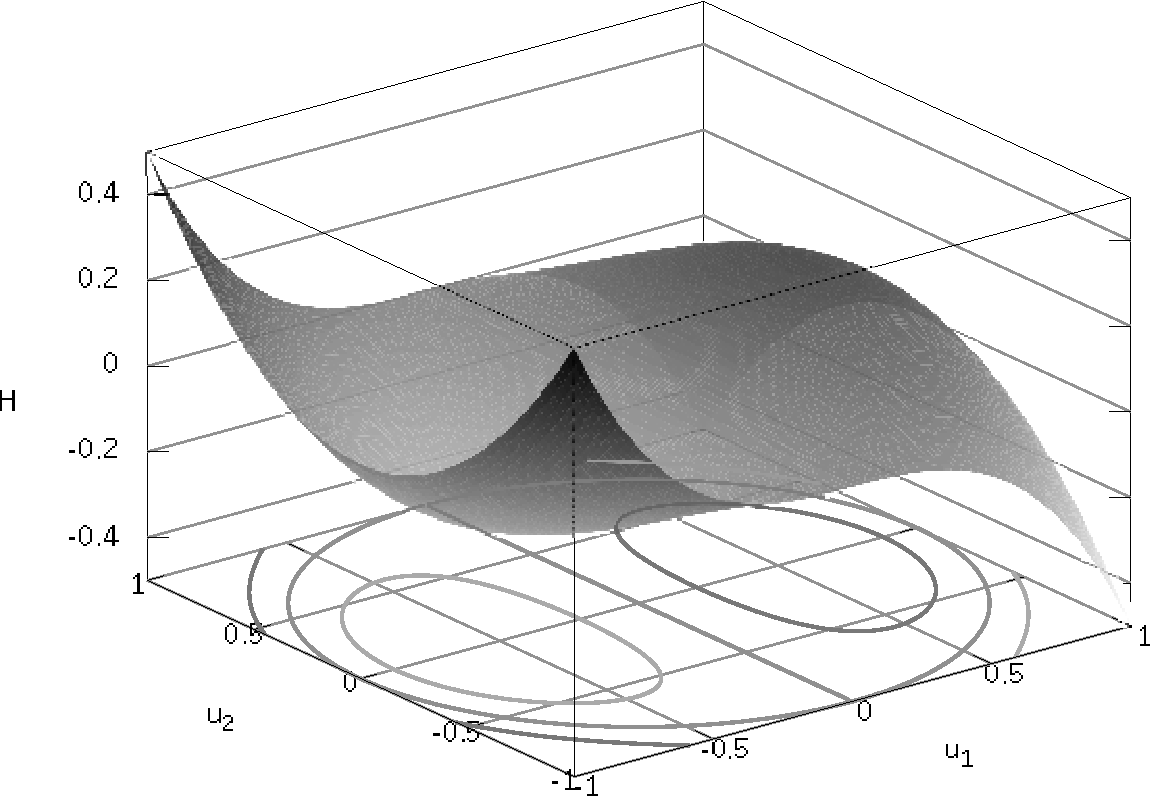
\includegraphics[width=\textwidth]{figures/h_surf}
\caption{Surface and contour plots of the averaged Hamiltonian in $u_1,u_2$ coordinates, as given in~\eqref{E:AvgH}. $I = 1$.}
\label{f:autoparam Hamiltonian}
\end{center}
% FIXME Surface should be restricted to $u_1^2 + u_2^2 \le 2 I$
\end{figure}

% FIXME The transformation below is not canonical and the variables z haven't been introduced
% Combining the transformations~\eqref{E:vector-trans}
% and~\eqref{E:sym-trans3} yields
% \begin{align} 
%  z_1 &= u_1 \cos \Theta + u_2 \sin \Theta &
%  z_2 &= \sqrt{2(I - u_1^2 - u_2^2)} \sin (\Theta/2)\notag\\
%  z_3 &= - u_1 \sin \Theta + u_2 \cos \Theta &
%  z_4 &= \sqrt{2(I - u_1^2 - u_2^2)} \cos (\Theta/2)
% \label{E:combin_transf}
% \end{align}
% where $\Theta= t + 2 \psi$ and ~\eqref{E:combin_transf} can be used to
% interpret the results of the averaged equations in terms of the
% original equations.

As $I$ varies, the system described by \eqref{E:vector-int} can display bifurcations. At exact resonance, by using the action-angle coordinates, we express the non-dissipative deterministic flow as
\begin{equation}
\label{E:hamilflow}
\begin{aligned}
\dot z_t^I(u) &= \bar{\nabla} K(z_t^I(u), I), \quad z_0^I(u)=u =(u_1,u_2)\\
\psi &= \int_{0}^{t} {D_{I} K(z_t^I(u), I) \ ds} + \psi_{0} \\ K
&= \text{constant} \in \reals, \quad I = \text{constant} \in \reals^+
\end{aligned}
\end{equation}
The dynamics in the $u$-space are completely integrable and represent a one parameter family of an one degree of freedom Hamiltonian system. The fixed points and the corresponding energy levels for the unperturbed system are given by
\begin{equation}
\begin{aligned}
A^\pm: (\bar u_1^{0}, \bar u_2^\pm) &= (0, \pm \sqrt{I}), \quad K_{A^\pm} = 0 \\
B^\pm: (\bar u_1^\pm, \bar u_2^{0}) & = (\pm \sqrt{\frac{I}{3}},0),  K_{B^\pm} = \pm\frac{I}{3}\sqrt{\frac{I}{3}}
\end{aligned}
\label{E:fixed-points}
\end{equation}
provided $ I \ge 0 $. The eigenvalues are given by $\pm \sqrt{\bar u_2^2-3 \bar u_1^2 }$. For $I > 0$, $A^\pm$ represent saddle points while $B^\pm$ represent center fixed points and at $I = 0$ all four fixed points coalesce at the origin and both the eigenvalues are zero. It follows from transformations~\eqref{E:combin_transf} that $0 \le u_1^2+u_2^2 \le I$. Hence, the domain of interest is restricted to the area within and including the heteroclinic orbits; the periodic orbits encircling the two elliptic fixed points and the heteroclinic orbits.

Note that at the origin, the reduced domain has a cusp since
\begin{align*}
K &= \frac{I}{3}\sqrt{\frac{I}{3}} & \text{and}&&\eval{\frac{dK}{dI}}_{I=0} &= 0.
\end{align*}

\section{Time-Averaging}
\label{S:T-Average}

We have pointed out that that there are three time-scales involved in our averaging problems. According to the theory presented in Section \ref{s:stochatic averaging theory}, the first step is to average the periodic fluctuations of the coefficients and obtain $\Tave$-averaged quantities as the precursors to the stochastically averaged drift and diffusion coefficients. Somewhat laborious calculations yield
\begin{equation}
\begin{aligned}
m_1(x) &\equiv \left(\Tave \left(F_1^2 + \mathfrak{f}_1 + \mathfrak{g}_1\right)\right)(x)\\
&=-\frac{1}{32R}\left( \left(x_4^2-x_2^2 \right)x_3+2 x_1 x_2 x_4\right)\left(6R\left( x_1^2+x_3^2 \right)-x_2^2-x_4^2\right) \\
&\quad -(\zeta_o+2\,\zeta_p) K +\frac12\mu x_3(x_2^2-x_4^2) - \mu x_1x_2x_4\\
m_2(x)&\equiv\left(\Tave \left(F_2^2 + \mathfrak{f}_2 + \mathfrak{g}_2\right)\right)(x)\\
&= 2 \sigma^2S_{\xi\xi}(1) -2\zeta_o(x_1^2+x_3^2) - \zeta_p(x_2^2 + x_4^2)
\end{aligned}
\label{E:drift1}
\end{equation}
\begin{equation}
\begin{aligned}
a_{11}(x) &\equiv \left(\Tave \left(\sigma\sigma^T\right)_{11}\right)(x)\\
&= \frac{1}{32}\sigma^2S_{\xi\xi}(1)\left(x_2^2 + x_4^2\right)^2\\
a_{12}(x) &\equiv \left(\Tave \left(\sigma\sigma^T\right)_{12}\right)(x)\\
&= \sigma^2S_{\xi\xi}(1) K\\
a_{22}(x) &\equiv \left(\Tave \left(\sigma\sigma^T\right)_{22}\right)(x)\\
&= 2\sigma^2S_{\xi\xi}(1)\left(x_1^2+x_3^2\right)
\end{aligned}
\label{E:diffusion1}
\end{equation}
The symplectic transformation of \eqref{E:combin_transf} provides a convenient geometric structure of the unperturbed integrable Hamiltonian problem. In $(u,K,I)$ coordinates, the drift \eqref{E:drift1} and diffusion \eqref{E:diffusion1} coefficients are
\begin{equation}
\begin{aligned}
m_1(u,y) &= -(\zeta_o + 2\zeta_p) K\\
&\quad + \frac{1}{8 R} \left(u_1^2+u_2^2-I \right) u_2 \left(u_1^2+u_2^2-I + 3 R \left( u_1^2+u_2^2 + \frac{8 \mu}{3} \right) \right) \\
&= -(\zeta_o + 2\zeta_p) K - \frac14 \left(8\mu + 3I\right) K \frac{u_2}{u_1} + \frac12\left(3 + \frac{1}{R}\right)K^2 \frac{u_2}{u_1^2}\\
m_2(u,y) &= 2[\sigma^2 S_{\xi\xi}(1) - \zeta_o I + 2 (\zeta_o - \zeta_p) K/u_1]
\end{aligned}
\label{E:drift2}
\end{equation}
\begin{equation}
\begin{aligned}
a_{11}(u,y) &=\frac{1}{8} \sigma^2 S_{\xi\xi}(1) \left(u_1^2 + u_2^2 - I \right)^2\\
&= \frac12 \sigma^2 S_{\xi\xi}(1) K^2 \frac{1}{u_1^2}\\
a_{12}(u,y) &= \sigma^2 S_{\xi\xi}(1) K\\
a_{22}(u,y) &= 2 \sigma^2S_{\xi\xi}(1) (u_1^2 + u_2^2)\\
&= 2 \sigma^2 S_{\xi\xi}(1) (I - 2 K/u_1).
\end{aligned}
\label{E:diffusion2}
\end{equation}
Since, there are certain advantages in the use of one form of $m_{i}(u,y)$ and $a_{ij}(u,y)$ over the other, we shall make use of either one of the forms in evaluating the diffusion coefficients.

To obtain a limiting generator for the martingale problem, we need an averaging operator where the averaging is done with respect to the invariant measure concentrated on the closed trajectories.

In the deterministic context Neistadt's condition ~\citep{neistadt75:_passag_throug_reson_in_two_frequen_probl, neistadt75:_averag_in_multi_frequen_system,lochak88:_multip_averag_for_class_system} ensures the existence of an average transverse force that drives the trajectories away from the resonance zones. For the stochastic case, it was shown~\citet{ramakrishnan00:_near_reson_motion_of_random} that even for the case when Neistadt's condition does not hold, passage of trajectories through resonance without getting captured can be ensured if appropriate conditions on the noise are satisfied.

Using \eqref{E:drift2} in the $\Aave$-averaging operator yields on each leaf $\Gamma_i$, for $y=(K,I) \in \Gamma_i$,
\begin{gather}
\begin{split}
\mathfrak b_1^i &= \frac{1}{\period_i(y)}\int_{0}^{\period_i(y)} m_1(u(t),y) dt\\
&= -(\zeta_o+2\zeta_p) K -\frac14 (8\mu + 3I) K \frac{1}{\period_i} \int_0^{\period_i} \frac{u_2(t)}{u_1(t)} dt\\
&\quad + \frac12 \Bigl(3 + \frac{1}{R} \Bigr) K^2
\frac{1}{\period_i} \int_{0}^{\period_i}
\frac{u_2(t)}{{u_1(t)}^2} dt\\
&= -(\zeta_o + 2\zeta_p) K
\end{split}
\label{E:drift h}\\
\begin{split}
\mathfrak b_2^i & = \frac{1}{\period_i(y)}\int_{0}^{\period_i(y)} m_2(u(t),y) dt\\
& = 2 [\sigma^2 S_{\xi\xi}(1) - \zeta_o I] + 4(\zeta_o-\zeta_p) K
\frac{1}{\period_i}\int_{0}^{\period_i}\frac{dt}{u_1(t)}\\
& = 2 [\sigma^2 S_{\xi\xi}(1) - \zeta_o I] + 4(\zeta_o-\zeta_p) K \frac{\INT_{i}^1}{\period_i}
\end{split}
\end{gather}
\begin{gather}
\begin{split}
\mathfrak a_{11}^i &= \frac{1}{\period_i(y)}\int_{0}^{\period_i(y)} a_{11}(u(t),y) dt\\
&= \frac12 \sigma^2 S_{\xi\xi}(1) K^2 \frac{1}{\period_i}\int_0^{\period_i}
\frac{1}{{u_1(t)}^2}dt\\
&= \frac12 \sigma^2 S_{\xi\xi}(1){K}^2 \frac{\INT_{i}^2}{\period_i}
\end{split}\\
\begin{split}
\Aa_{12}^{i} &= \frac{1}{\period_i(y)}\int_{0}^{\period_i(y)} a_{12}(u(t),y)dt\\
&= \sigma^2 S_{\xi\xi}(1) K
\label{E:diffusion hi}
\end{split}
\\
\begin{split}
\Aa_{22}^i &= \frac{1}{\period_i(y)} \int_0^{\period_i(y)} a_{22}(u(t),y)dt\\
&= 2 \sigma^2 S_{\xi\xi}(1) \left(I - \frac{2 K}{\period_i} \int_0^{\period_i} \frac{1}{u_1(t)}dt \right)\\
&= 2 \sigma^2 S_{\xi\xi}(1) (I - 2 K \frac{\INT_i^1}{\period_i})
\end{split}
\end{gather}
We want to put these $\gen_i$'s together to get a Markov process on $\Graph$ with generator $\gen^\dagger_\Graph$ with domain $\mathscr{D}^\dagger_\Graph$, where $\Graph$ has a shape of an \emph{arrowhead}. For notational convenience, we also define $f_i \equiv f\big|_{\mathfrak{I}_i}$ for all $1\le i\le 2$. From the results of \citet{freidlin98:_random_pertur_nonlin_oscil}, and \citet{sowers03:_stoch_averag_near_homoc_orbit}, it is clear the gluing conditions, which we need to specify at the interior edges, solely depend on the diffusion coefficients $\Aa_{jk}^{i}$. To this end, we define
\[
\mathring{\Aa}_{jk}^{i}(y)\equiv \Aa_{jk}^{i}(y) \, \period(y)
\]
The limiting domain for the graph valued process is
\begin{multline}
\mathscr{D}_\Graph^\dagger = \left\{f \in C(\Graph) \cap C^2(\cup_{i=1}^2 \mathfrak I_i): \lim_{y \to (K(\mathfrak c_i),I(\mathfrak c_i))}(\gen_i f_i)(y) \text{ exists } \forall \, i\right.\\
\left.\lim_{I \to I^*} (\gen_i f_i)(y) = 0\; \forall\, i, \sum_{i=1}^2 \; \sum_{j=1}^2\,\left\{ \sum_{k=1}^2 \mathring{\Aa}_{jk}^{i}(y) \frac{\partial f_i(y)}{\partial y_k}\right\} \nu_j \Big|_{y = \Order} = 0\right\}
\label{E:dom-graph}
\end{multline}
where $\nu$ is the outward normal vector to the boundary $\partial\Gamma_i$. The gluing condition is the last term in the expression above. The gluing condition can be simplified by making use of the fact that the period
is asymptotically equivalent to $\period(y) \sim \ln |K|$ as $K \to 0$, thus it can be verified that
\[
\lim_{K \to 0} \mathring{\Aa}_{11}^{i}(y) < \infty, \quad \lim_{K \to 0} \mathring{\Aa}_{12}^{i}(y)= 0, \quad \text{and} \quad \lim_{K \to 0} \mathring{\Aa}_{22}^1(y) = \lim_{K \to 0} \mathring{\Aa}_{22}^2(y)
\]
and in addition the vertex~$\Order \equiv [0,I^*]$ consistes of a
vertical line ($\nu_2 = 0$). Hence, the limiting domain for the graph
valued process simplifies to
\begin{multline}
\mathscr{D}_\Graph^\dagger = \left\{f\in C(\Graph)\cap C^2(\cup_{i=1}^2\mathfrak{I}_i): \lim_{y \to \left(K(\mathfrak{c}_i),I(\mathfrak{c}_i)\right)}(\gen_i f_i)(y) \text{ exists } \forall \, i, \right.\\
\left. \lim_{I \to I^*}(\gen_i f_i)(y)=0 \, \forall \, i, \text{ and } \sum_{i=1}^2 \{\pm\} (\mathring{\Aa}_{11}^{i}\,\frac{\partial f_i}{\partial y_1})(\Order) = 0 \right\}
\label{E:dom-graph-simplified}
\end{multline}
where the `$+$' sign is taken if the coordinate $h$ on the leg
$\mathfrak{I}_i$ is greater than $0$~(the value of $y_1(=h)$ at the
vertex~${\Order}$) and the `$-$' sign is taken otherwise. Then for $f\in
\mathscr{D}_\Graph^\dagger$, the generator is
\begin{equation}
(\gen^\dagger_\Graph f)(y) = \sum_{j=1}^2 \mathfrak{b}_j^i(y) \frac{\partial f_i}{\partial y_j}(y) + \frac12 \sum_{j,k=1}^2 \Aa_{jk}^i(y) \frac{\partial^2 f_i}{\partial y_j \partial y_k}(y)
\label{E:gen-graph}
\end{equation}
for all $y \in \bar{\mathfrak I}_i$, where the averaged drift and
diffusion coefficients on each leg $\mathfrak I_i$ are evaluated
making use of the calculations in Appendix~\ref{A:autoparam
path_integrals}. The period of the orbits is the same
\[
\period_1 = \period_2 = \frac{4}{\sqrt{\lambda_1 (\lambda_2 - \lambda_3)}} K(\kappa)
\]
% FIXME: Many of the coefficients are the same ``in the valley'' and ``on the hill''. To save space, should not repeat them.
\begin{enumerate}
\item $u_1 < 0, \quad H < 0$: The integrals are calculated along the paths which correspond to the ``oscillations in the valley''.
% FIXME: ``Tidy-up'' these equations & decide if some of the calculations steps should be removed}
\begin{equation}
\mathfrak b_1^1 = -(\zeta_o + 2 \zeta_p) H \label{e:b1 valley}\\
\end{equation}
\begin{align*}
\mathfrak b_2^1 &= 2 [\sigma^2 S_{\xi\xi}(1) - \zeta_o I]\notag\\
&\quad + 8 (\zeta_p - \zeta_o) \frac{1}{T_1 \sqrt{\lambda_1 \left(\lambda_2-\lambda_3 \right)}} \left[-\lambda_1 \lambda_2 K(\kappa) + {\lambda_1\left(\lambda_2-\lambda_3 \right)} E(\kappa) \right]\notag\\
& = 2[\sigma^2 S_{\xi\xi}(1) - \zeta_o I] +2 \left(\zeta_o - \zeta_p\right) \lambda_1 \lambda_2\notag\\
&\quad - 2 \left(\zeta_o - \zeta_p\right) \lambda_1 \left(\lambda_2 - \lambda_3\right) \frac{E(\kappa)}{K(\kappa)}\notag\\
& = 2 [\sigma^2 S_{\xi\xi}(1) - \zeta_o I] - 4 (\zeta_o - \zeta_p) \frac{H}{\lambda_2 \kappa^2} \left[ \kappa^2 - \alpha^2 + \alpha^2 \frac{E(\kappa)}{K(\kappa)}\right]\notag\\
& = 2 [\sigma^2 S_{\xi\xi}(1) - \zeta_o I] + 4 (\zeta_o - \zeta_p) \frac{|H|}{\lambda_2 \kappa^2} \left[ \kappa^2 - \alpha^2 + \alpha^2 \frac{E(\kappa)}{K(\kappa)}\right]
\end{align*}
\begin{align*}
\Aa_{11}^1 &= \frac{1}{6}{\sigma}^2 S_{\xi\xi}(1) \frac{\lambda_1^2}{T_1 \sqrt{\lambda_1 \left(\lambda_2 - \lambda_3 \right)}} \big[\left(\lambda_2 - \lambda_3 \right)^2 \kappa^2\\
&\quad + \left(-\lambda_3^2 + 2 \lambda_3 \lambda_2 + 2 \lambda_2^2\right)\big] K(\kappa) \\
&\quad -\frac{1}{3} {\sigma}^2 S_{\xi\xi}(1)\frac {\lambda_1^2}
{T_1\,\sqrt {\lambda_1\left(\lambda_2-\lambda_3\right)} }\left
(\lambda_2-\lambda_3\right) \big[\left(\lambda_2 - \lambda_3 \right)\kappa^2\\
&\quad + \left(\lambda_2 + 2\lambda_3\right)\big] E(\kappa)\\
& = \frac{1}{24}\,{\sigma}^2S_{\xi\xi}(1){\lambda_1}^2
\left[\left(\lambda_2-\lambda_3\right)^2{\kappa}^2 + \left
(-{\lambda_3}^2 + 2 \lambda_3 \lambda_2 + 2 {\lambda_2}^2\right)\right]\\
&\quad -\frac{1}{12}\,{\sigma}^2S_{\xi\xi}(1){\lambda_1}^2\left
(\lambda_2-\lambda_{{ 3}}\right)\left[\left
(\lambda_2-\lambda_{{ 3}}\right){\kappa}^2+\left
(\lambda_2+2\,\lambda_3\right)\right] \frac{E(\kappa)}{K(\kappa)}\\
& = \frac{1}{6} \sigma^2 S_{\xi\xi}(1) \left(\frac{H}{\lambda_2 \kappa^2} \right)^2 \biggl[ \left(3 \kappa^4 - 6 \alpha^2 \kappa^2 + 2 \alpha^4 + \alpha^4 \kappa^2 \right)\\
&\quad -2\,{\alpha}^2\left(-3\,{\kappa}^2+{\alpha}^2+{\alpha}^2{\kappa}^2\right)\frac{E(\kappa)}{K(\kappa)} \biggr]
\end{align*}
\[
\Aa_{12}^1 = \sigma^2 S_{\xi\xi}(1) H
\]
\begin{align*}
\Aa_{22}^1 &= 2 \sigma^2 S_{\xi\xi}(1){I}\\
&\quad + 8 \sigma^2 S_{\xi\xi}(1) \frac{1}{T_2 \sqrt{\lambda_1\left(\lambda_2 - \lambda_3 \right)}}\left[ -\lambda_1 \lambda_2 K(\kappa) + {\lambda_1\left(\lambda_2 - \lambda_3 \right)} E(\kappa) \right]\\
& = 2 \sigma^2 S_{\xi\xi}(1)I - 2 \sigma^2 S_{\xi\xi}(1) \lambda_1 \lambda_2 + 2 \sigma^2 S_{\xi\xi}(1) \lambda_1 \left(\lambda_2 - \lambda_3\right) \frac{E(\kappa)}{K(\kappa)}\\
& = 2 \sigma^2 S_{\xi\xi}(1) I - 4 \sigma^2 S_{\xi\xi}(1) \frac{|H|}{\lambda_2 \kappa^2} \left[\kappa^2 - \alpha^2 + \alpha^2 \frac{E(\kappa)}{K(\kappa)}\right]
\end{align*}
Where $K(\kappa), E(\kappa)$ are complete elliptic integrals of the first and the second kinds with the modulus
\[
\kappa^2 \equiv \frac{\lambda_3(\lambda_2 - \lambda_1)}{\lambda_1(\lambda_2 - \lambda_3)} > 0.
\]
\item $u_1 > 0, \quad K > 0$: In this case, the integrals are calculated along the paths which correspond to the ``oscillations on the hill''.
\begin{equation}
\label{e:b1 hill}
\mathfrak{b}_1^2 = -(\zeta_o+2\zeta_p) H
\end{equation}
\begin{align*}
\mathfrak b_2^2 &= 2[\sigma^2 S_{\xi\xi}(1) - \zeta_o I]\\
& + 8 (\zeta_o - \zeta_p)\,\frac{1}{T_2\,\sqrt{\lambda_1\left(\lambda_2 - \lambda_3 \right)}}\left[ -\lambda_1 \lambda_2 K(\kappa) + {\lambda_1 \left(\lambda_2 - \lambda_3 \right)} E(\kappa) \right]\\
&= 2 [\sigma^2 S_{\xi\xi}(1) - \zeta_o I] - 2 \left(\zeta_o - \zeta_p\right) \lambda_1 \lambda_2\\
&\quad + 2 \left(\zeta_o - \zeta_p\right) \lambda_1 \left(\lambda_2 - \lambda_3 \right) \frac{E(\kappa)}{K(\kappa)}\\
&= 2[\sigma^2 S_{\xi\xi}(1) - \zeta_o I] + 4 (\zeta_o-\zeta_p) \frac{H}{\lambda_2{\kappa}^2} \left[ \kappa^2 - \alpha^2 + \alpha^2 \frac{E(\kappa)}{K(\kappa)}\right]\\
&= 2[\sigma^2 S_{\xi\xi}(1) - \zeta_o I] + 4 (\zeta_o-\zeta_p) \frac{|H|}{\lambda_2{\kappa}^2} \left[ \kappa^2 - \alpha^2 + \alpha^2 \frac{E(\kappa)}{K(\kappa)}\right]
\end{align*}
\begin{align*}
\Aa_{11}^2 &= \frac{1}{6}{\sigma}^2 S_{\xi\xi}(1) \frac{\lambda_1^2}{T_2 \sqrt{\lambda_1 \left(\lambda_2 - \lambda_3 \right)}} \Big[\left(\lambda_2 - \lambda_3 \right)^2 \kappa^2\\
&\quad + \left(-{\lambda_3}^2 + 2 \lambda_3 \lambda_2 + 2 \lambda_2^2\right)\Big] K(\kappa)\\
&\quad -\frac{1}{3}\,{\sigma}^2S_{\xi\xi}(1)\frac {\lambda_1^2} {T_2\,\sqrt {\lambda_1\left(\lambda_2 - \lambda_3\right)}}\left(\lambda_2 - \lambda_3\right)\Big[\left(\lambda_2 - \lambda_3\right)\kappa^2\\
&\quad + \left(\lambda_2 + 2 \lambda_3 \right)\Big] E(\kappa)\\
& = \frac{1}{24}\,{\sigma}^2S_{\xi\xi}(1){\lambda_1}^2 \left[\left(\lambda_2-\lambda_3\right)^2 \kappa^2 + \left(-{\lambda_3}^2 + 2 \lambda_3 \lambda_2 + 2 \lambda_2^2\right)\right]\\
&\quad -\frac{1}{12}\,{\sigma}^2S_{\xi\xi}(1){\lambda_1}^2\left(\lambda_2-\lambda_{{ 3}}\right)\left[\left(\lambda_2 - \lambda_3 \right){\kappa}^2 + \left(\lambda_2 + 2 \lambda_3 \right)\right] \frac{E(\kappa)}{K(\kappa)}\\
& = \frac{1}{6}\,{\sigma}^2S_{\xi\xi}(1) \,\left(\frac{H}{\lambda_2{\kappa}^2} \right)^2 \,\biggl[\left( 3 \kappa^4 - 6 \alpha^2 \kappa^2 + 2 \alpha^4 + \alpha^4 \kappa^2\right)\\
&\quad -2 \alpha^2 \left(-3 \kappa^2+\alpha^2 + \alpha^2 \kappa^2\right) \frac{E(\kappa)}{K(\kappa)}\biggr]
\end{align*}
\[
\Aa_{12}^2 = \sigma^2 S_{\xi\xi}(1) H
\]
\begin{align*}
\Aa_{22}^2 & = 2 \sigma^2 S_{\xi\xi}(1){I}-8 \sigma^2 S_{\xi\xi}(1) \frac{1}{T_2 \sqrt{\lambda_1\left(\lambda_2-\lambda_3 \right)}}\big[ - \lambda_1 \lambda_2 K(\kappa)\\
&\quad + {\lambda_1\left(\lambda_2-\lambda_3 \right)} E(\kappa) \big]\\
& =2\,{\sigma}^2S_{\xi\xi}(1){I} + 2 {\sigma}^2 S_{\xi\xi}(1)\lambda_1\lambda_2 - 2 \sigma^2 S_{\xi\xi}(1) \lambda_1 \left(\lambda_2-\lambda_3 \right)\frac{E(\kappa)}{K(\kappa)}\\
& = 2 \sigma^2 S_{\xi\xi}(1) I - 4 \sigma^2 S_{\xi\xi}(1) \frac{|H|}{\lambda_2 \kappa^2} \left[\kappa^2 - \alpha^2 + \alpha^2 \frac{E(\kappa)}{K(\kappa)}\right]
\end{align*}
\end{enumerate}

We derive the gluing conditions, by determining asymptotic values as $h \to 0$. The asymptotic values of the three roots are
\begin{align*}
\lambda_1&=\sqrt I - \epsilon/I & \lambda_2&=2\epsilon/I & \lambda_3&=-\sqrt I - \epsilon/I.
\end{align*}
The period is asymptotically equivalent to $\period(y) \sim \ln |H|$ as $H \to 0$. This yields $\lim_{h \to 0}\mathring{\mathfrak{b}}_1^i = 0$.
Furthermore,
\begin{align}
\lim_{h \to 0} \mathring\Aa_{11}^{i}({\Order})&\equiv\lim_{h \to 0} \left(\Aa_{11}^i \period_i\right) \notag\\
&= - \frac{1}{6}\,{\sigma}^2\,S_{\xi\xi}(1) \lim_{h \to 0} \left(\lambda_1  \lambda_{3}^2 \right) \lim_{\kappa^\prime \to 0} \left({\kappa^\prime}^2 \, \ln \frac{4}{\kappa^{\prime}} \right) \notag\\
&\quad + \frac{1}{3}\,{\sigma}^2S_{\xi\xi}(1) \lim_{h \to 0} \left(\lambda_1 \lambda_{3}^2 \right) \lim_{\kappa \to 1} \left(\left\{2-{\kappa}^2\right\}\, E(\kappa)\right) \notag\\
& = \sigma^2 S_{\xi\xi}(1) \frac{I \sqrt{I}}{3} \geq 0\label{E:lim drift_11}
\end{align}
Hence $-\dot f_1(y) +\dot f_2(y) = 0$.
Note that the values of $\mathring{\mathfrak b}_2^i$, $\mathring\Aa_{12}^i$ and $\mathring\Aa_{22}^i$ in the limit $k \to 0$ all approach infinity.

The complete domain within which the FPE is specified is shown in Figure~\ref{F:domain}. This domain is described as having two ``leaves'' with a common edge at $K=0$. The edge at $K=0$ is called the gluing edge.

\begin{figure}
\begin{center}
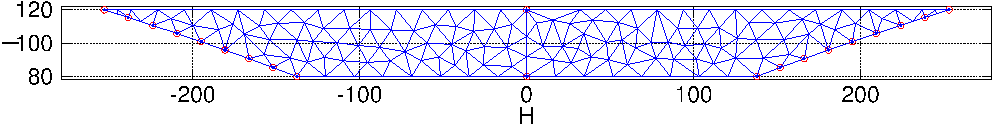
\includegraphics[width=\textwidth*7/8]{figures/domain_crop}
\caption{Example of domain within which the FPE is specified. A finite element triangulation of the domain is also shown.}
\label{F:domain}
\end{center}
\end{figure}

A set of illustrative values for $\mathring{\mathfrak a}$ is shown in Figures~\ref{F:a11_circ},~\ref{F:a12_circ} and~\ref{F:a22_circ}. Likewise, Figures~\ref{F:b1_circ} and~\ref{F:b2_circ} show values for $\mathring{\mathfrak b}$. Note that at points where no data is shown (ie. on the line $K=0$), the coefficients are unbounded, although certain coefficients do have a value in the limit $K \to 0$.

\begin{figure}
\begin{center}
\psfrag{a11*t}{$\mathring{\mathfrak a}_{11}$}
\psfrag{H}{$y_1$}
\psfrag{I}{$y_2$}
% 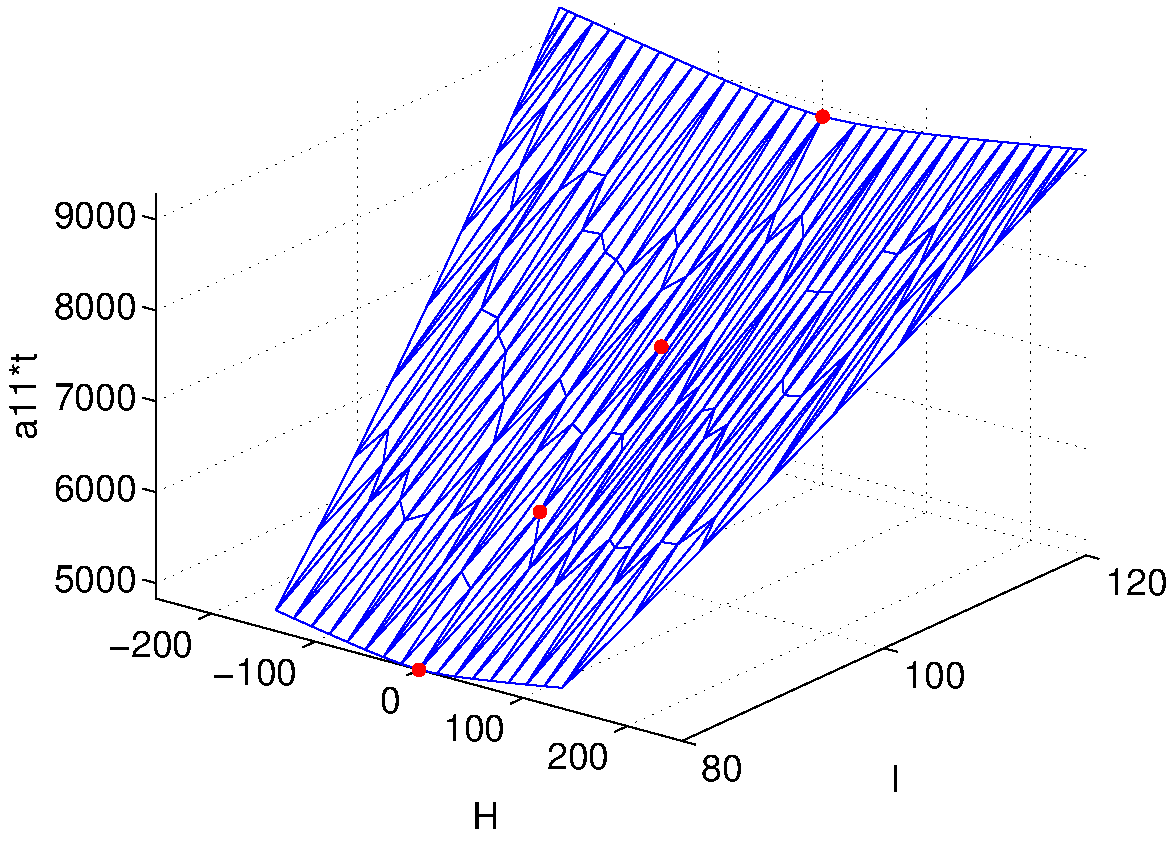
\includegraphics[clip=true,viewport=1in 1in 7in 5.5in,width=\textwidth*7/8]{figures/a11_circ}
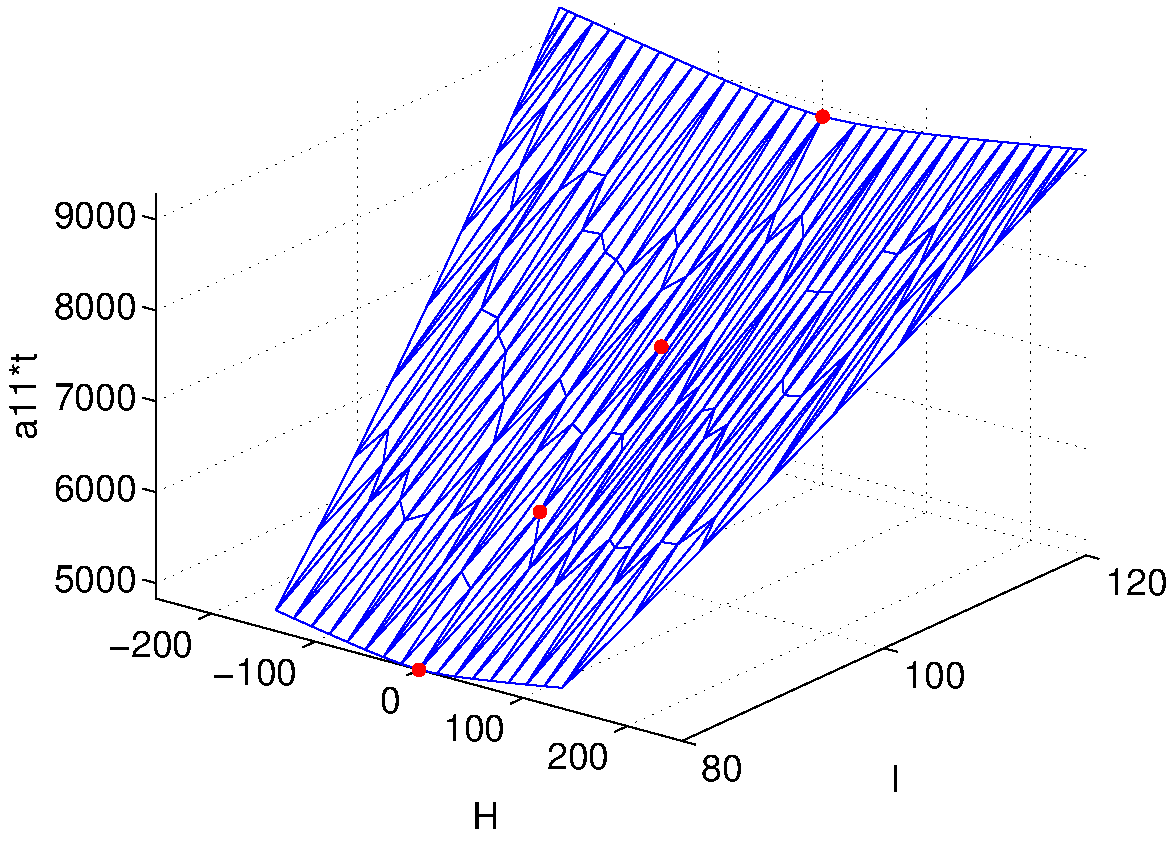
\includegraphics[width=\textwidth*7/8]{figures/a11_circ}
\caption{Example of numeric values for $\mathring{\mathfrak a}_{11}$. Circles denote points where the value is only defined by equation~\eqref{E:lim drift_11}.}
\label{F:a11_circ}
\end{center}
\end{figure}
\begin{figure}
\begin{center}
\psfrag{a12*t}{$\mathring{\mathfrak{a}}_{12}$}
\psfrag{H}{$y_1$}
\psfrag{I}{$y_2$}
% 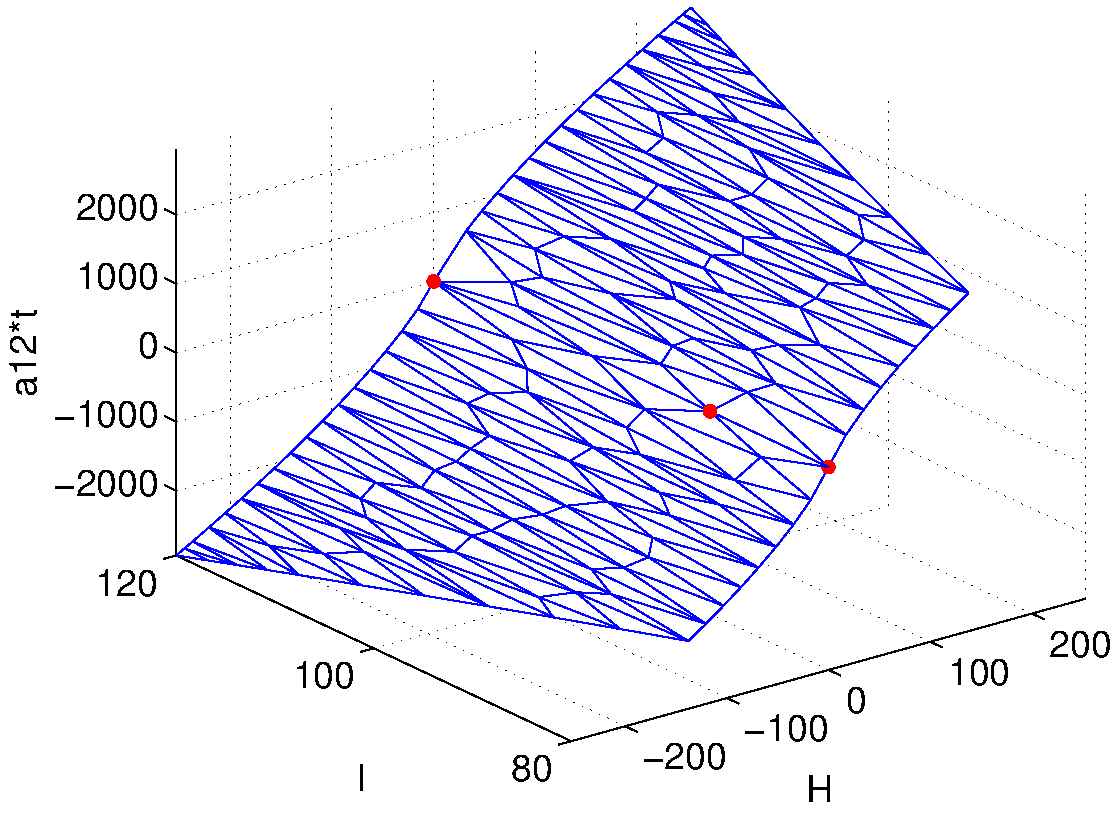
\includegraphics[clip=true,viewport=1in 1in 7in 5.5in,width=\textwidth*7/8]{figures/a12_circ}
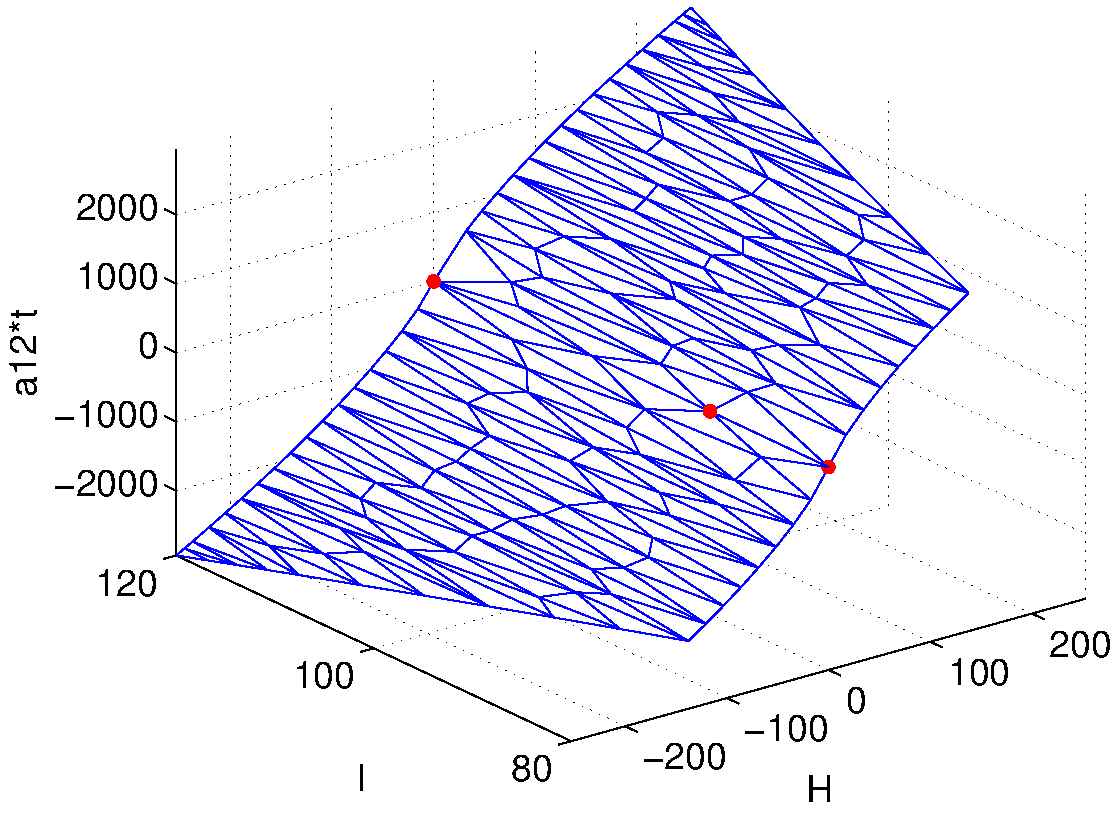
\includegraphics[width=\textwidth*7/8]{figures/a12_circ}
\caption{Example of numeric values for $\mathring{\mathfrak a}_{12}$. Circles denote points where the value is only defined by $\lim_{y_2 \to 0} \mathring{\mathfrak a}_{12} = 0$.}
\label{F:a12_circ}
\end{center}
\end{figure}
\begin{figure}
\begin{center}
\psfrag{a22*t}{$\mathring{\mathfrak{a}}_{22}$}
\psfrag{H}{$y_1$}
\psfrag{I}{$y_2$}
% 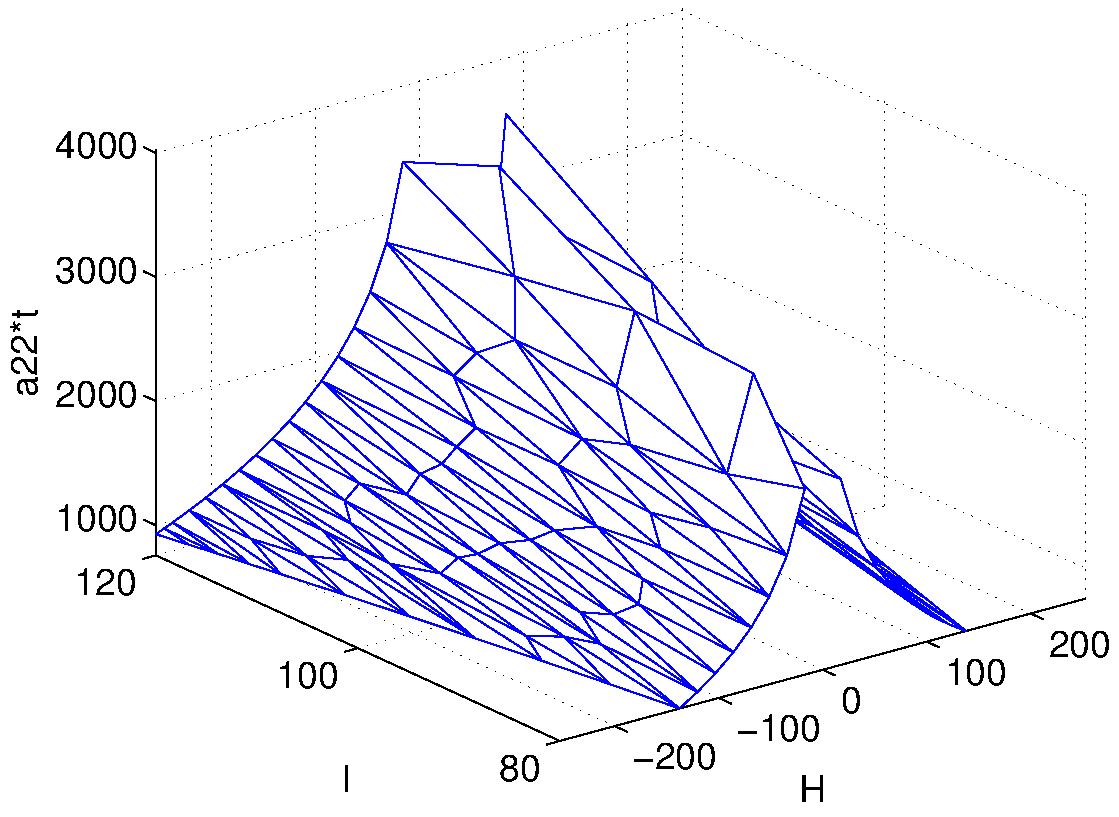
\includegraphics[clip=true,viewport=1in 1in 7in 5.5in,width=\textwidth*7/8]{figures/a22_circ}
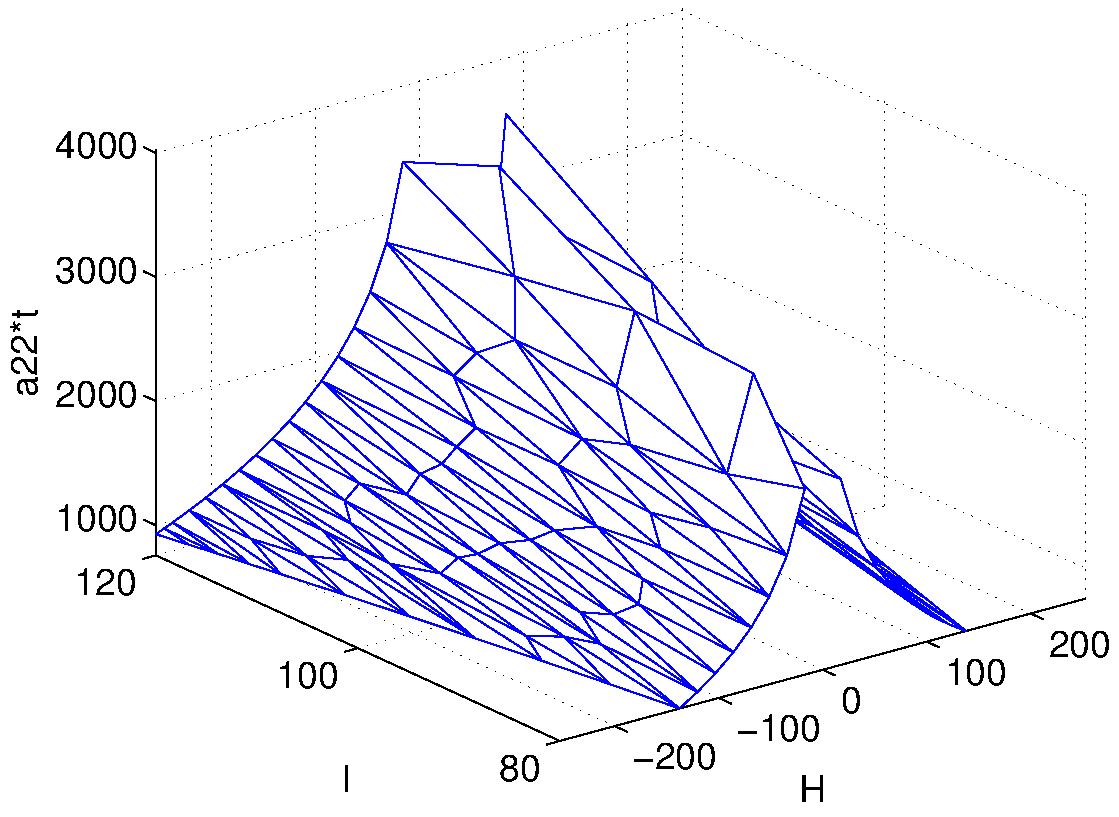
\includegraphics[width=\textwidth*7/8]{figures/a22_circ}
\caption{Example of numeric values for $\mathring{\mathfrak a}_{22}$. On the gluing edge, the value goes to infinity.}
\label{F:a22_circ}
\end{center}
\end{figure}
\begin{figure}
\begin{center}
\psfrag{b1*t}{$\mathring{\mathfrak{b}}_1$}
\psfrag{H}{$y_1$}
\psfrag{I}{$y_2$}
% 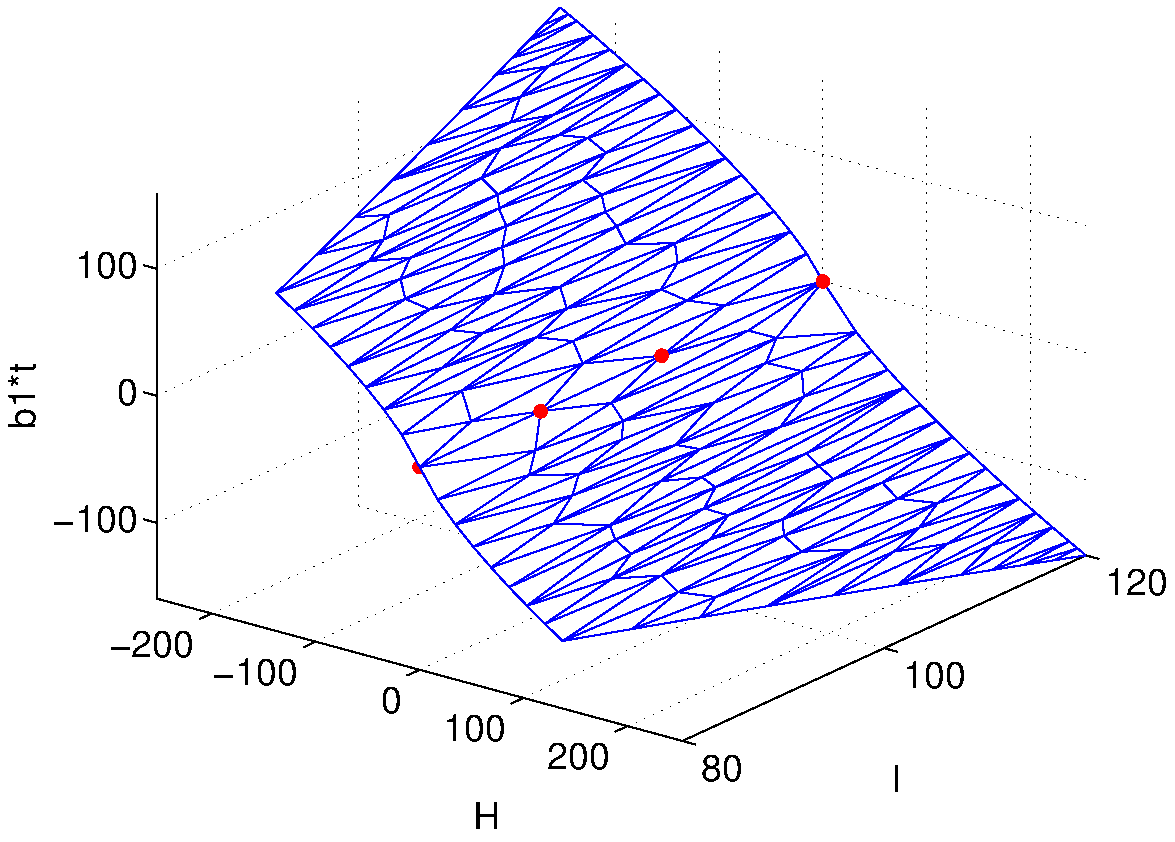
\includegraphics[clip=true,viewport=1in 1in 7in 5.5in,width=\textwidth*7/8]{figures/b1_circ}
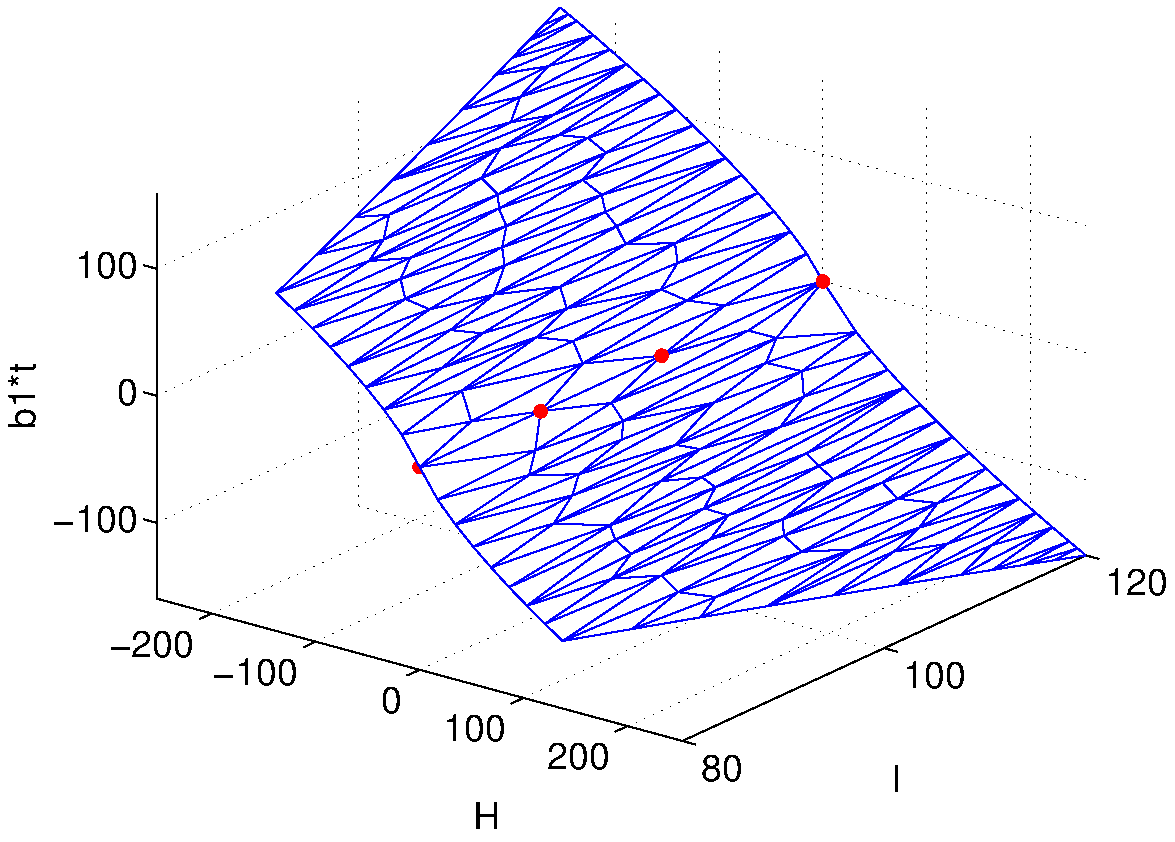
\includegraphics[width=\textwidth*7/8]{figures/b1_circ}
\caption{Example of numeric values for $\mathring{\mathfrak b}_1$. Circles denote points where the value is only defined by $\lim_{y_1 \to 0} \mathring{\mathfrak b}_1 = 0$.}
\label{F:b1_circ}
\end{center}
\end{figure}
\begin{figure}
\begin{center}
\psfrag{b2*t}{$\mathring{\mathfrak b}_2$}
\psfrag{H}{$y_1$}
\psfrag{I}{$y_2$}
% 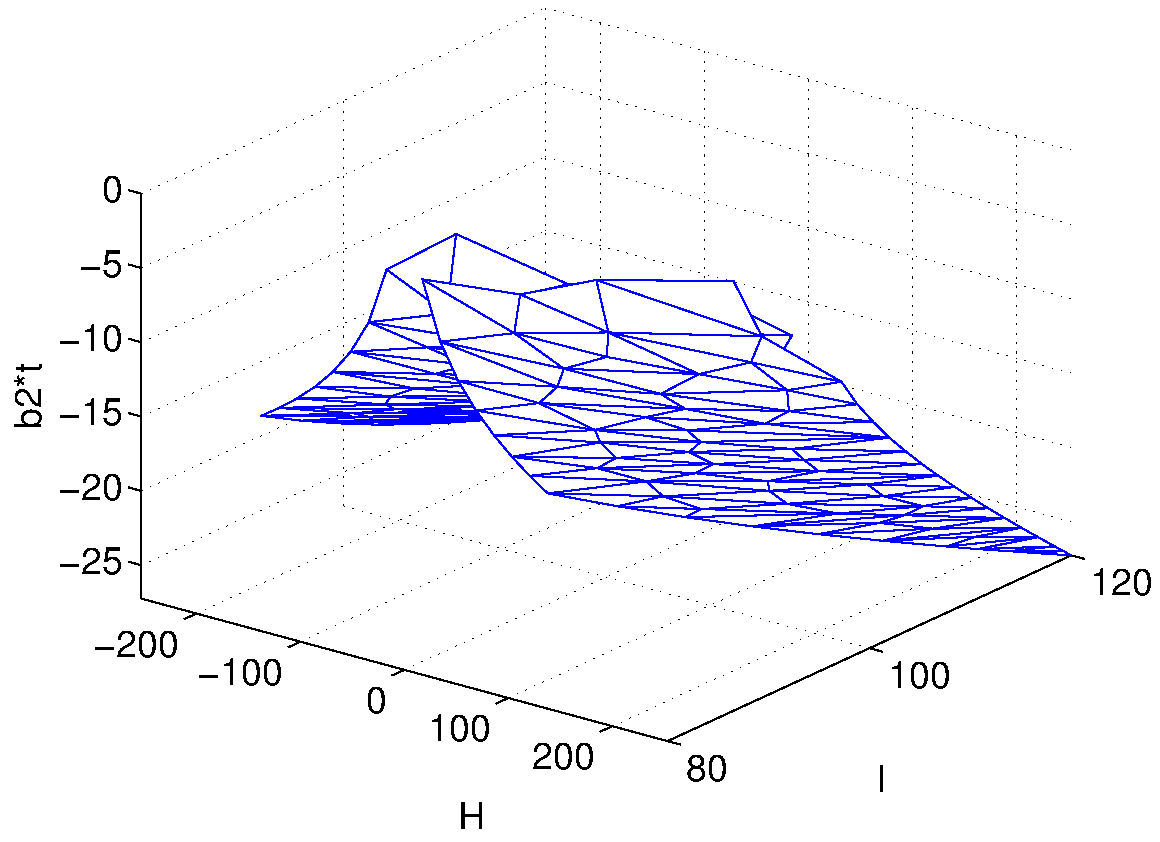
\includegraphics[clip=true,viewport=1in 1in 7in 5.5in,width=\textwidth*7/8]{figures/b2_circ}
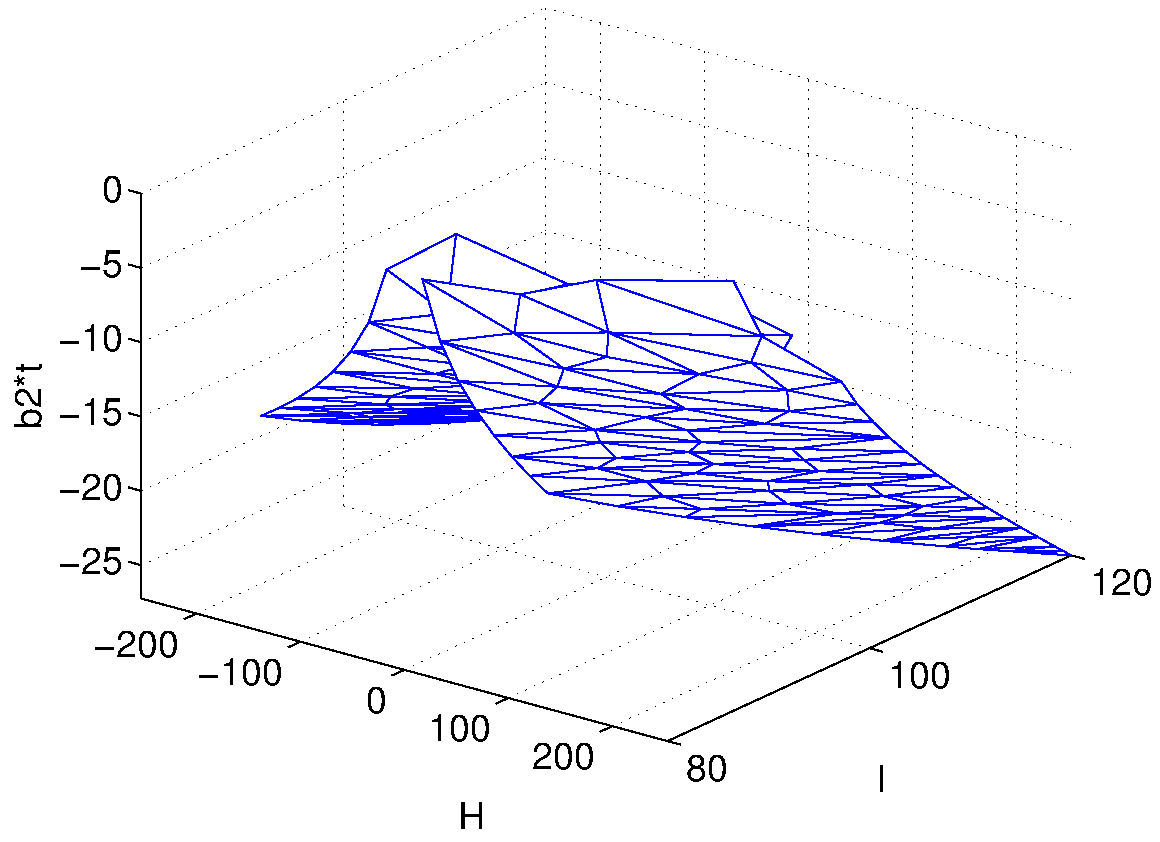
\includegraphics[width=\textwidth*7/8]{figures/b2_circ}
\caption{Example of numeric values for $\mathring{\mathfrak b}_2$. On the gluing edge, the value goes to infinity.}
\label{F:b2_circ}
\end{center}
\end{figure}

% FIXME Add figure showing the period

\section{Conclusions}

This chapter has shown how it is possible to analyze the stochastic motion of a pair of oscillators auto-parametrically coupled. In broad terms, the methodology used to achieve this was the same as for the wave model in \ref{c:sgwaves}. Differences exist in the details however. 1:2 resonance was imposed for the autoparametric problem whereas the wave model was near 1:1 resonance. The reduced domain of the autoparametric system contains two leaves, whereas the surface waves model has three. With regards to calculating averaged drift and diffusion coefficients, completely analytic results have been obtained for the autoparametric system, leading to formulas that contain elliptic integrals.

In the next chapter, the analysis of the autoparametric oscillator continues. Now that the generator of the reduced Markov process and its domain have been completely characterized in a weak sense, it becomes possible to derive a partial differential equation governing the evolution of probability density functions for the autoparametric oscillators. This equation will be derived in the next chapter, and it will be solved numerically.

%%% Local Variables: 
%%% mode: latex
%%% TeX-master: "main"
%%% End: 
